\documentclass[t,11pt,british,english, top=1.0in]{beamer}
\usepackage{hyperref}
\usepackage{graphics}
\usepackage{amsmath}
\usepackage{amssymb}
\usepackage{natbib}
        %You can use the package \textbf{pgfpages} 
        %to arrange your slides for printing. This is also explained
        %in the \textbf{beamer} documentation.

\newcommand{\tensor}[1]{\overline{\overline{#1}}}
\newcommand{\tautens}{\tensor{\tau}}

\setbeamerfont{framesubtitle}{size=\normalsize}
\setbeamerfont{framesubtitle}{size=\normalsize}
%\setbeamertemplate{frametitle}[default][center]
%\setbeamersize{text margin left=6mm}

\usetheme{Madrid}
\usecolortheme{orchid}

%gets rid of bottom navigation bars
\setbeamertemplate{footline}[page number]{}
\setbeamertemplate{headline}{}

%gets rid of navigation symbols
\setbeamertemplate{navigation symbols}{}

\begin{document}
\title{Data Handling for Researchers\\\vspace*{5mm}\small Christian Jacobs, Matthew Piggott, Gerard Gorman, David Ham\\\vspace*{5mm}4 March 2014}
\author{} 
\date{} 

\frame{\titlepage} 

\frame{
   \frametitle{Course Outcomes}
   \begin{itemize}
   \item Understand {\color{red}what data is} and {\color{red}why it is important}.\vspace*{3mm}
   \item Understand the need to {\color{red}backup}, {\color{red}compress}, and {\color{red}encrypt} data.\vspace*{3mm}
   \item Be aware of {\color{red}best practices}.\vspace*{3mm}
   \item Be aware of the {\color{red}tools} available for analysis and testing.\vspace*{3mm}
   \item Know the basics of version-controlled file {\color{red}repositories}.\vspace*{3mm}
   \end{itemize}
}

\frame{
   \frametitle{What is data?}
   \framesubtitle{Definition} 
   \begin{itemize}
    \item Data is a {\color{red}set of values} corresponding to one or more {\color{red}quantitative} or {\color{red}qualitative variables}.
    \vspace*{6mm}
    \item Examples:
      \begin{itemize}
        \item Sea levels measured every hour at a fixed location\vspace*{1mm}
        \item Speed of a car throughout time\vspace*{1mm}
        \item Metadata (= data that describes other data) for webpages\vspace*{1mm}
        \item Wind velocity at different locations in the UK\vspace*{1mm}
        \item Depth of a particle settling in a water tank, measured at various times.
      \end{itemize}
     \vspace*{4mm}
    \item Data can come from {\color{red}existing sources}, may be {\color{red}derived} from several data sets, or a {\color{red}new independent data set} can be generated.
   \end{itemize}
}

\frame{
   \frametitle{What is data?}
   \framesubtitle{More examples} 
   Values of particle concentration in space following a volcanic eruption:
   \begin{figure}[H]
      \centering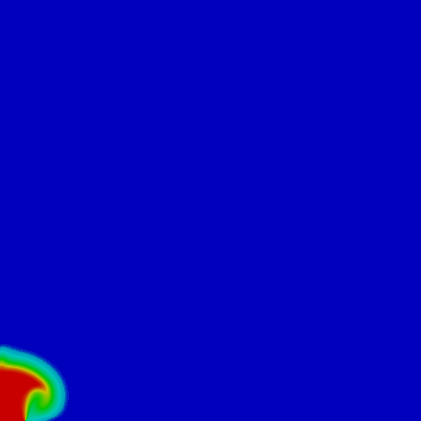
\includegraphics[width=0.32\columnwidth]{images/eruption_vfrac_10s.png}\hspace*{0.5mm}
      \centering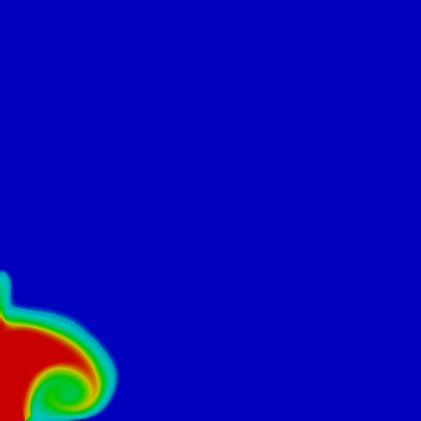
\includegraphics[width=0.32\columnwidth]{images/eruption_vfrac_30s.png}\hspace*{0.5mm}
      \centering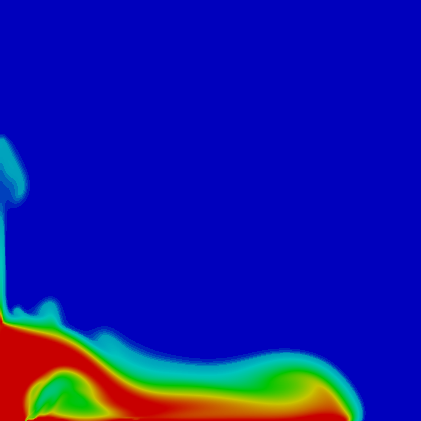
\includegraphics[width=0.32\columnwidth]{images/eruption_vfrac_70s.png}
      
      \centering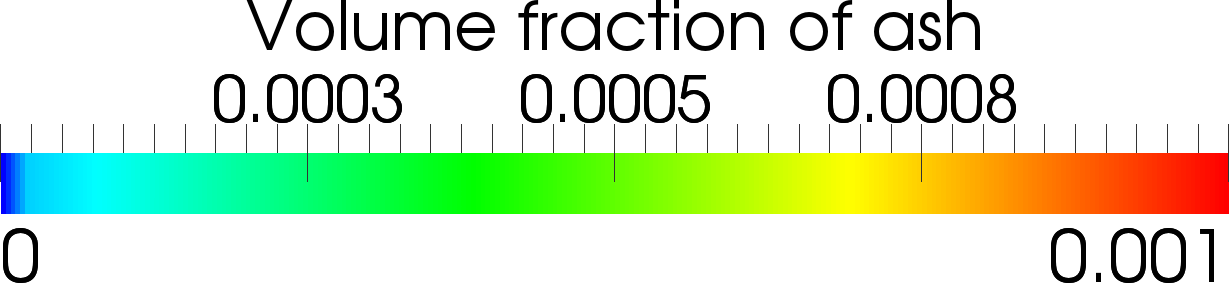
\includegraphics[width=0.3\columnwidth]{images/vfrac_legend.png}
   \end{figure}
}


\frame{
   \frametitle{What is data?}
   \framesubtitle{More examples} 
   Air density at various temperatures. Data from the Density page on Wikipedia.
   \begin{figure}[H]
      \centering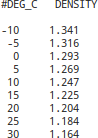
\includegraphics[width=0.25\columnwidth]{images/density.png}
   \end{figure}
}

\frame{
   \frametitle{What is data?}
   \framesubtitle{More examples} 
   Numerical solution error against grid spacing:
   \begin{figure}[H]
      \centering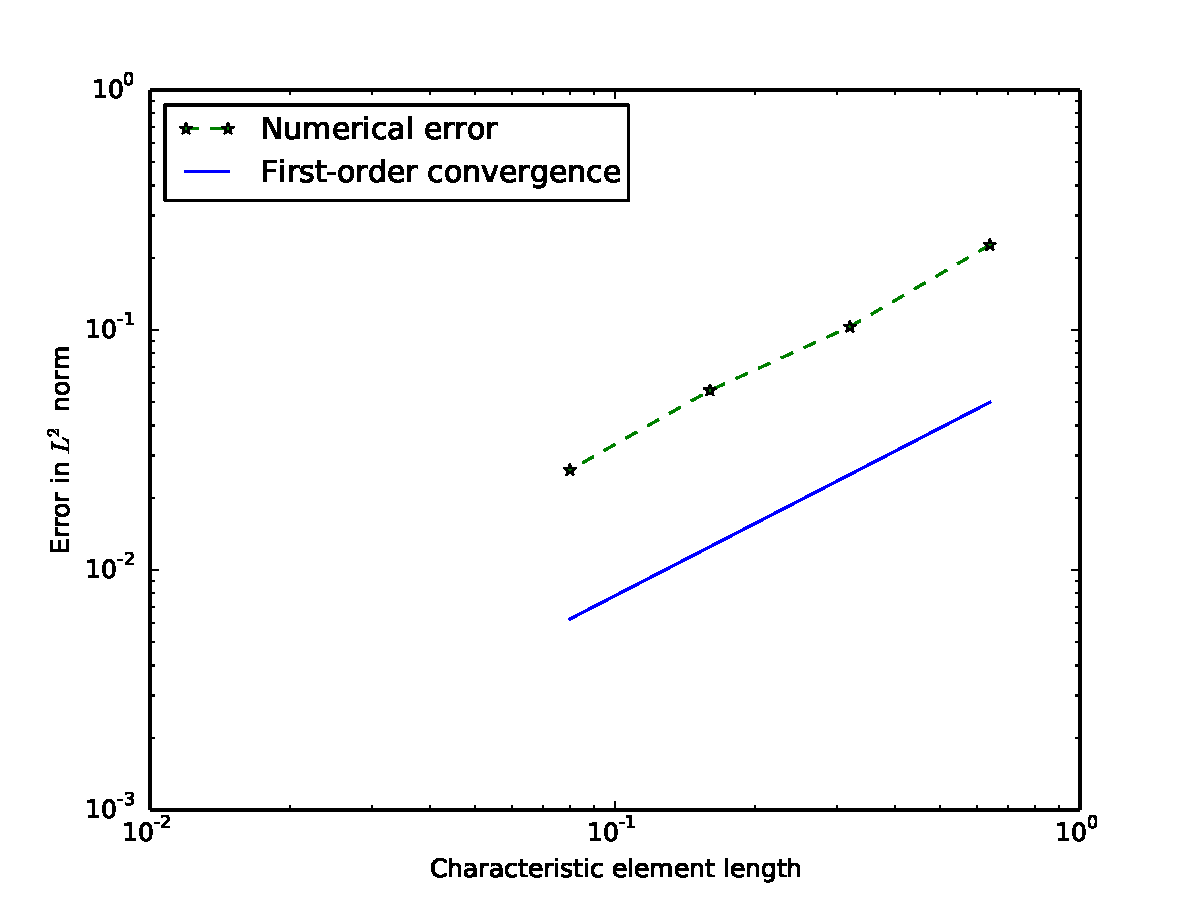
\includegraphics[width=0.765\columnwidth]{images/convergence.pdf}
   \end{figure}
}


\frame{
   \frametitle{Why is data important?}
   %\framesubtitle{Definition} 
   \begin{itemize}

    \item Allows {\color{red}new scientific discoveries} to be made.\vspace*{3mm}
    
    \item Journals and research councils are encouraging the {\color{red}sharing} of data to:
       \begin{itemize}
          \item promote research output,
          \item minimise the duplication of data,
          \item increase transparency and accountability, 
          \item allow fellow researchers to scrutinise and evaluate the data. 
       \end{itemize} \vspace*{3mm}
 
   \item The effective handling and management of all research data plays an important role in each of these processes. 
   
   \end{itemize}
}

\frame{
   \frametitle{Why is data important?}
    ``Notice of Retraction''\\\vspace*{3mm}
    ``For the article by Bertoia et al, ``Implications of New Hypertension Guidelines in the United States,'' [$\ldots$] the authors discovered an error in the code for analyzing the data.''. \\\vspace*{3mm}
    ``Consequently, the sample size was twice as large as it should have been (24989 instead of 10198).''\\\vspace*{3mm}
    ``For these reasons, \textit{Hypertension} requested that the authors resubmit a corrected version of this manuscript.''\\\vspace*{3mm}
    doi: 10.1161/​HYP.0b013e318269bc7a
}

\frame{
   \frametitle{Why is data important?}
    ``By reanalysing inaccurately presented data of Kerr et al. (2006), we refute their claims that area-corrected species richness of endemic Madagascan birds and mammals increases toward the Equator and is best explained by environmental factors, and that the rainforest mid-domain effect (MDE) Lees et al. (1999) demonstrated is artefactual.''\\\vspace*{3mm}
    doi: 10.1111/j.1461-0248.2007.01040.x
}

\frame{
   \frametitle{Issues to consider}
   \framesubtitle{Data provenance} 
   \begin{itemize}
    \item {\color{red}Where} did the data originally come from? Is there a {\color{red}chain} that can be traced back to the origin of the data? \vspace*{3mm}
    \item Can it be {\color{red}trusted}? (Is the author list available? Reputable journal?)\vspace*{3mm}
    \item Is it {\color{red}reproducible}?\vspace*{3mm}
    \item Has the data already been used successfully? Any reported issues?
   \end{itemize}
}

\frame{
   \frametitle{Issues to consider}
   \framesubtitle{Licensing} 
   \begin{itemize}
    \item {\color{red}Who} can use the data, and {\color{red}how}?\vspace*{3mm}
    \item Who owns the {\color{red}copyright}? Are you allowed to publish it or use it in your thesis?
    \vspace*{3mm}
    \item Any user {\color{red}licence}? Creative Commons licences are becoming more popular and offer more freedom.\vspace*{3mm}
    \item Data produced when employed by a Government agency may be under {\color{red}Crown Copyright}. The copyright does not belong to an individual, and is instead under the control of Her Majesty's Stationery Office (HMSO) - see \texttt{www.nationalarchives.gov.uk/information-management}.\vspace*{6mm}
    \item \textbf{You need to know the answer to these points before you base any of your work on this data.}
   \end{itemize}
}

\frame{
   \frametitle{Issues to consider}
   \framesubtitle{File formats} 
   \begin{itemize}
    \item Using {\color{red}standardised, open-source} file formats makes your data {\color{red}portable} (between computers and operating systems) and facilitates sharing of data by other researchers. \vspace*{3mm}
    \item Comma-Separated Value ({\color{red}CSV}): a commonly-used format for simple data sets. Values in a single row are separated by commas. CSV files can contain multiple rows, thereby forming a table. \vspace*{3mm}
    \item eXtensible Markup Language ({\color{red}XML}): each piece of data is encapsulated in a tag which annotates/describes it. \vspace*{3mm}
    \item Network Common Data Form ({\color{red}NetCDF}): commonly used in numerical climate and ocean models.
   \end{itemize}
}


\frame{
   \frametitle{Issues to consider}
   \framesubtitle{File formats -- CSV} 
   \begin{figure}[H]
      \centering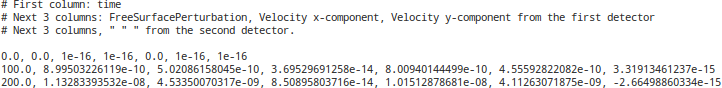
\includegraphics[width=1\columnwidth]{images/csv.png}
   \end{figure}
}

\frame{
   \frametitle{Issues to consider}
   \framesubtitle{File formats -- XML} 
   \begin{figure}[H]
      \centering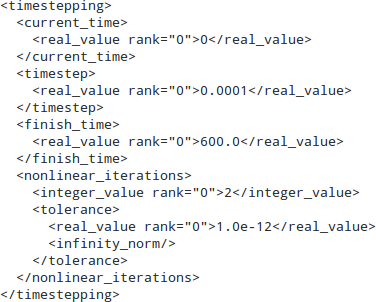
\includegraphics[width=0.7\columnwidth]{images/xml.png}
   \end{figure}
}

\frame{
   \frametitle{Issues to consider}
   \framesubtitle{File formats -- NetCDF} 
   \begin{itemize}
    \item A binary file format commonly used in numerical climate and ocean models. \vspace*{3mm}
    \item It is ``self-describing'': header information and metadata are automatically included.\vspace*{3mm}
    \item Several NetCDF file readers are readily available.\vspace*{3mm}
    \item \texttt{www.unidata.ucar.edu/software/netcdf}
   \end{itemize}
}

\frame{
   \frametitle{Issues to consider}
   \framesubtitle{Storage options}
   \begin{itemize}
    \item Optical media (CDs ~700 MB, DVDs ~4.7 GB, Blu-ray 25+ GB) and flash drives - for small files e.g. presentations, theses, papers.\vspace*{3mm}
    \item Magnetic media (hard drives) - for larger files (e.g. simulation output).\vspace*{3mm}
    \item Cloud services (e.g. Dropbox, Google Drive).\vspace*{3mm}
    \item Always maintain a good {\color{red}file hierarchy} and {\color{red}naming convention} when storing data files.
   \end{itemize}
}

\frame{
   \frametitle{Issues to consider}
   \framesubtitle{Backing up}
   \begin{itemize}
    \item \textbf{The importance of regularly backing up data cannot be stressed enough!}\vspace*{3mm}
    \item What if your hard drive failed right now? What if your computer (and any connected backup device) was stolen?\vspace*{3mm}
    \item Storage space is reasonably cheap.\vspace*{3mm}
    \item Always keep {\color{red}several regular backups}, far apart from each other (not in the same building).\vspace*{3mm}
    \item Know the Imperial College data backup policy.\vspace*{6mm}
    \item imperial.ac.uk/ict/services/computerroom/file\_and\_backup\_services
   \end{itemize}
}


\frame{
   \frametitle{Issues to consider}
   \framesubtitle{Encryption}
   \begin{itemize}
    \item Be aware of responsibilities to encrypt {\color{red}sensitive information}.\vspace*{3mm}
    \item Encrypting emails: Pretty Good Privacy (PGP) keys. \texttt{www.pgp.com}\vspace*{3mm}
    \item Encrypting hard drives: TrueCrypt (Windows, Linux, Mac OS), eCryptfs (Linux).\vspace*{6mm}
    
    \item \footnotesize{The 'Climatic Research Unit email controversy': ``The Climatic Research Unit email controversy (also known as "Climategate")[2][3] began in November 2009 with the hacking of a server at the Climatic Research Unit (CRU) at the University of East Anglia (UEA) by an external attacker. [...] Climate change critics and others denying the significance of human caused climate change argued that the emails showed that global warming was a scientific conspiracy, in which they alleged that scientists manipulated climate data and attempted to suppress critics.''\\
    http://en.wikipedia.org/wiki/Climatic\_Research\_Unit\_email\_controversy}
   \end{itemize}
}

\frame{
   \frametitle{Issues to consider}
   \framesubtitle{Big Data}
   \begin{itemize}
    \item {\color{red}Big Data} is one of the key challenges in data science.\vspace*{3mm}
    \item Involves data sets that are {\color{red}extremely large}, thereby creating additional difficulties when analysing them.\vspace*{3mm}
    \item Need novel and efficient tools to help tackle this issue.\vspace*{3mm}
    \item Data Science Institute at Imperial.
   \end{itemize}
}

\frame{
   \frametitle{Creating and manipulating data}
   \framesubtitle{Tools}
   \begin{itemize}
    \item Data sets are often {\color{red}merged}, {\color{red}manipulated}, and {\color{red}generated} using computer programs or scripts.\vspace*{3mm}
    \item Often written in MATLAB or Python.\vspace*{3mm}
   \end{itemize}
}

\frame{
   \frametitle{Creating and manipulating data}
   \framesubtitle{Source code examples}
   \footnotesize
   Example from \texttt{www.programming4scientists.com}:
   \vspace*{3mm}

   \centering
   \begin{tabular}{p{4.5cm}|l}
   FUNCTION comppoly(x) & FUNCTION ComparePolynomials(x)\\
   float y1, y2 & //DECLARE VARIABLES, PARAMETERS\\
   float a1=0.1, b1=0.3, a2=2.1, b2=5.3, c=0.22 & float y\_line, y\_quadratic\\
   y1 = a1*x + b1 & float lineParam = [0.1, 0.3]\\
   y2 = a1*x\textasciicircum2 + b2*x + c & float quadParam = [2.1, 5.3, 0.22]\\
   return(y2$>$y1) & \\
   END FUNCTION & //CALCULATE THE LINE AND QUADRATIC\\
    & VALUES AT X\\
    & y\_line = lineParam[0]*x + lineParam[1]\\
    & y\_quadratic = quadParam[0]*x\textasciicircum2 + quadParam[1]*x\\
    &  + quadParam[2]\\
    & \\
    & //COMPARE THE FUNCTIONS, RETURNING\\
    & A LOGICAL\\
    & return(y\_line $>$ y\_quadratic)\\
    & END FUNCTION
   \end{tabular}
}

\frame{
   \frametitle{Creating and manipulating data}
   \framesubtitle{Commenting and documenting}
   \begin{itemize}
    \item Always {\color{red}comment} and {\color{red}document} your code to help yourself and others to understand how to use it.\vspace*{3mm}
    \item Use sensible variable names.\vspace*{3mm}
    \item Use {\color{red}metadata} to document the name of the author, the date the data was created, any terms of use, etc.
   \end{itemize}
}

\frame{
   \frametitle{Creating and manipulating data}
   \framesubtitle{Quality assurance}
   \begin{itemize}
    \item Test programs for {\color{red}correctness} in order to have confidence in the results.\vspace*{3mm}
    \item {\color{red}Regression testing} - identifies new faults that have been introduced from changes to the code.\vspace*{3mm}
    \item Programs can break even without changes to the source code (e.g. compiler faults).\vspace*{3mm}
    \item The data itself should also be tested using {\color{red}verification} and {\color{red}validation} techniques.
   \end{itemize}
}

\frame{
   \frametitle{Creating and manipulating data}
   \framesubtitle{Quality assurance -- Buildbot}
   Buildbot (\texttt{buildbot.net}): An automated continuous testing framework. The code is tested after any change is made.
   \begin{figure}[H]
      \centering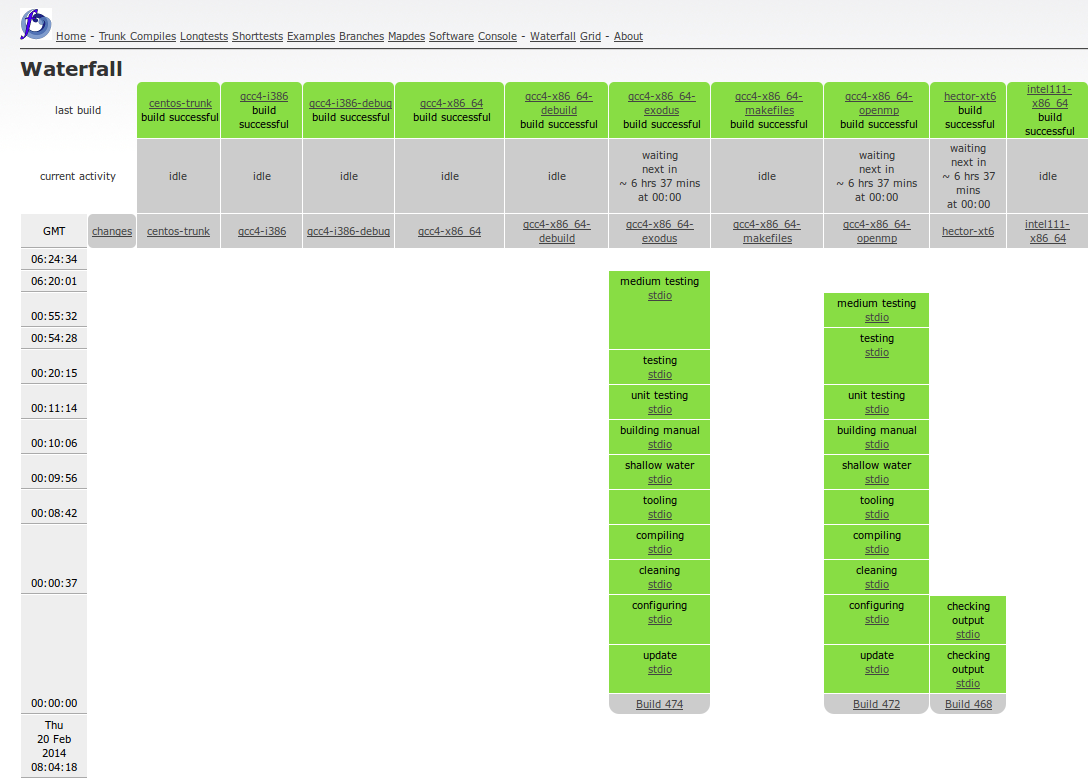
\includegraphics[width=1\columnwidth]{images/buildbot.png}
   \end{figure}
}

\frame{
   \frametitle{Creating and manipulating data}
   \framesubtitle{Version control systems}
   \begin{itemize}
    \item Used to {\color{red}keep track of changes} to data, and the programs used to generate data.\vspace*{3mm}
    \item Facilitates {\color{red}team development}.\vspace*{3mm}
   \begin{figure}[H]
      \centering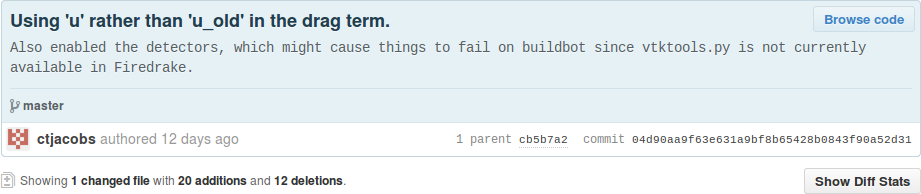
\includegraphics[width=0.9\columnwidth]{images/commit.png}
   \end{figure}\vspace*{-3mm}
   \begin{figure}[H]
      \centering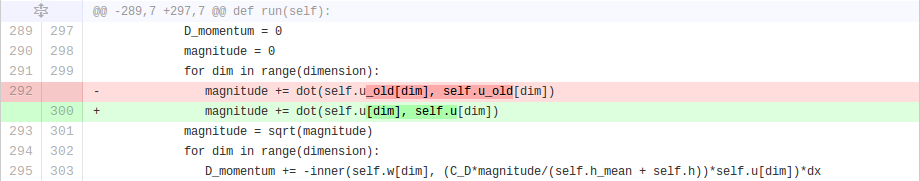
\includegraphics[width=0.9\columnwidth]{images/diff.png}
   \end{figure}\vspace*{-3mm}
   \end{itemize}
}

\frame{
   \frametitle{Creating and manipulating data}
   \framesubtitle{Version control systems --- Motivation}
   \small
   \begin{itemize}
      \item Many people choose to keep track of the different versions of a file by simply copying the current state of the file into a separate folder each time they want to record that change.
      \item This is very {\color{red}error prone}. Easy to overwrite files accidentally or forgetting to make a note of what exactly was changed. Extra work to merge different changes together.
   \end{itemize}
   \begin{figure}[H]
      \centering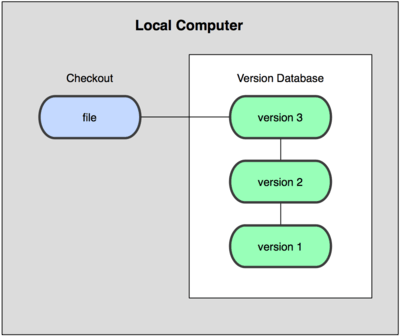
\includegraphics[width=0.4\columnwidth]{images/version_control_localonly.png}
   \end{figure}\vspace*{-3mm}
   \tiny{Image by Scott Chacon, used under the Attribution-NonCommercial-ShareAlike 3.0 Unported license.}
}

\frame{
   \frametitle{Creating and manipulating data}
   \framesubtitle{Version control systems --- Centralised}
   \begin{itemize}
      \item A {\color{red}server} stores all the files and the version history.
      \item Each time the file's state is saved (`{\color{red}committed}'), a log message must be written. This also gets stored on the server.
      \item Useful when multiple people are working on the same file.
      \item Requires a {\color{red}connection to the server} to commit changes.
   \end{itemize}
   \begin{figure}[H]
      \centering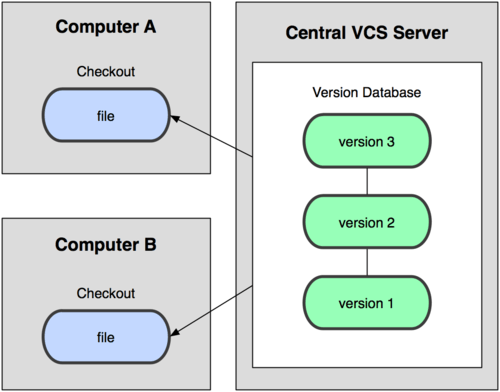
\includegraphics[width=0.45\columnwidth]{images/version_control_centralised.png}
   \end{figure}\vspace*{-3mm}
   \tiny{Image by Scott Chacon, used under the Attribution-NonCommercial-ShareAlike 3.0 Unported license.}
}

\frame{
   \frametitle{Creating and manipulating data}
   \framesubtitle{Version control systems --- Distributed}
   \begin{itemize}
      \item The checkout is effectively a {\color{red}full backup} of the data.
      \item Does not require a connection to the server to commit changes.
   \end{itemize}
   \begin{figure}[H]
      \centering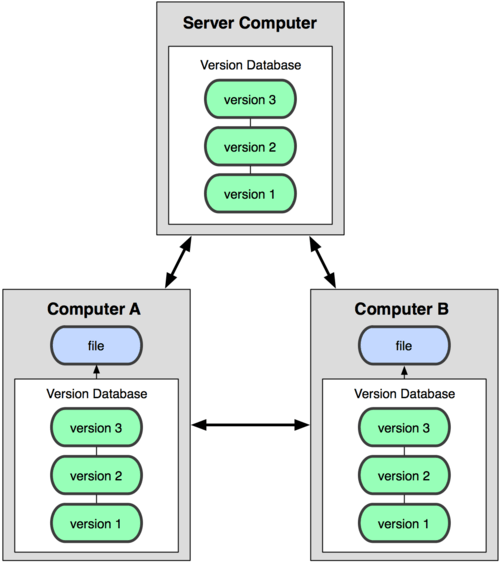
\includegraphics[width=0.4\columnwidth]{images/version_control_distributed.png}
   \end{figure}
   \tiny{Image by Scott Chacon, used under the Attribution-NonCommercial-ShareAlike 3.0 Unported license.}
}

\frame{
   \frametitle{Creating and manipulating data}
   \framesubtitle{Version control systems --- Tracking Differences}
   \begin{itemize}
      \item When committing or `checking-in' changes, the differences between the files you are committing and the files from the previous version are recorded in the history log.
   \end{itemize}
   \begin{figure}[H]
      \centering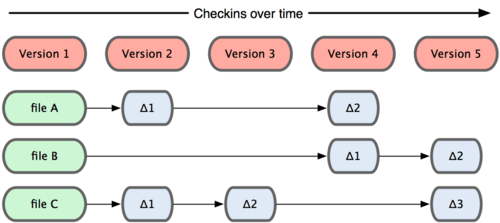
\includegraphics[width=0.75\columnwidth]{images/version_control_differences.png}
   \end{figure}
   \tiny{Image by Scott Chacon, used under the Attribution-NonCommercial-ShareAlike 3.0 Unported license.}
}

\frame{
   \frametitle{Creating and manipulating data}
   \framesubtitle{Version control systems --- Examples}
   \begin{itemize}
    \item Examples: {\color{red}Subversion} (\texttt{subversion.apache.org}), {\color{red}Bazaar} (\texttt{bazaar.canonical.com}), {\color{red}Git} (\texttt{git-scm.com})\vspace*{3mm}
    \item Some services such as GitHub (\texttt{www.github.com}) and Bitbucket (\texttt{www.bitbucket.org}) offer free Git-based repositories.
   \end{itemize}
}

\frame{
   \frametitle{Creating and manipulating data}
   \framesubtitle{Exercise 1}
   \begin{itemize}
    \item Let's work our way through a set of Git exercises created by GitHub: \texttt{http://try.github.io}\vspace*{7mm}
    \item Initialise a verson-controlled repository using \texttt{git init}\vspace*{3mm}
    \item Add files to the repository using \texttt{git add <file\_name\_here>}\vspace*{3mm}
    \item Remove files from the repository using \texttt{git rm <file\_name\_here>}\vspace*{3mm}
    \item Commit any changes using \texttt{git commit -a} (the \texttt{-a} adds the modified files to the staging area, and then commits the changes - see the documentation for more information.)
   \end{itemize}
}

\frame{
   \frametitle{Creating and manipulating data}
   \framesubtitle{Exercise 2}
   \begin{itemize}
    \item Set up an account at \texttt{www.github.com}.\vspace*{3mm}
    \item Download the Git for Windows tool here: \texttt{windows.github.com}\vspace*{3mm}
    \item Set up a new repository called \texttt{data-handling-course}.\vspace*{3mm}
    \item Download the files from the following web address to your repository's folder (Desktop/GitHub/data-handling-course): \\
    amcg.ese.ic.ac.uk/$\sim$ctj10/data-handling-course\vspace*{3mm}
    \item Run the program \texttt{plot\_rainfall.m}. A plot of the mean rainfall will be saved as \texttt{rainfall\_plot.png}. Add and commit this file to your data-handling-course repository.\vspace*{3mm}
    \item Run the regression test program \texttt{test\_rainfall.m}.
   \end{itemize}
}

\frame{
   \frametitle{Creating and manipulating data}
   \framesubtitle{Exercise 2 - Continued}
   \begin{itemize}
    \item Note 1: Any work that you store in a GitHub repository is made public (unless you pay for a private repository).
    \item Note 2: As an alternative, Bitbucket offers unlimited free {\color{red}private} repositories.
    \item Note 3: You can delete the GitHub account at any time under the account settings page.
   \end{itemize}
}

\frame{
   \frametitle{Creating and manipulating data}
   \framesubtitle{Exercise 2 - Continued}
   \begin{itemize}
    \item If you need additional functionality: {\color{red}Git for Windows} (\texttt{msysgit.github.io}), or {\color{red}gitk} for Linux (\texttt{git-scm.com/docs/gitk}).\vspace*{3mm}
    \item These aren't tied to just GitHub or Bitbucket.
   \end{itemize}
}

\frame{
   \frametitle{Additional resources}
   \begin{itemize}
    \item The UK Data Archive: \texttt{www.data-archive.ac.uk}\vspace*{3mm}
    \item The Software Sustainability Institute: \texttt{www.software.ac.uk}\vspace*{3mm}
    \item Software Carpentry: \texttt{software-carpentry.org}\vspace*{3mm}
    \item Digital Curation Centre: \texttt{www.dcc.ac.uk}\vspace*{3mm}
    \item Information Commissioner's Office: \texttt{ico.org.uk}\vspace*{3mm}
    \item IASSIST: \texttt{www.iassistdata.org}\vspace*{10mm}
    
    \item G. Wilson et al. (2014). Best Practices for Scientific Computing, PLoS Biol 12(1). doi: 10.1371/journal.pbio.1001745\vspace*{2mm}
    \item L. Hatton, A. Roberts (1994). How accurate is scientific software?, Software Engineering, IEEE Transactions, 20(10):785--797. doi: 10.1109/32.328993
   \end{itemize}
}

\end{document}
